\appendix

\chapter{Algoritmo de Ramificación y Acotamiento}
\label{app:bb}

\noindent
El Algoritmo \ref{algo:bb} presenta una versión rudimentaria del algoritmo de ramificación y
acotamiento. El rendimiento de este método depende en gran parte de la elección del subproblema
\eqref{p1c9:alg:BB_loop} pues partir de su solución podemos obtener cotas que nos permitan podar
subárboles lo más pronto posible. En la práctica, también debemos tomar en cuenta estrategias de
selección que permitan paralelizar la solución de los problemas relajados, o que minimicen la
sobrecarga computacional de ``saltar'' de un subproblema a otro.

Además del problema de selección de los nodos, también se encuentra el de creación de estos nodos.
En la línea \eqref{p1c9:alg:branch} ramificamos $S_i$ usando una de las técnicas más básicas: elegir
$x_j^i$ fraccionario y generar $S_{i0}$, $S_{i1}$ a partir de los cortes válidos $x_j \leq
\floor{x_j^i}$ y $x_j \geq \ceil{x_j^i}$. En realidad, existen muchas otras estrategias de corte,
tales como los cortes de Gomory, cortes SOS1, cortes de pseudo costos, cortes fuertes, cortes de
mochila, etcétera.

Implementaciones comerciales y de código abierto extienden el algoritmo de Ramificación y
Acotamiento a partir de otros esquemas. Es común que estas cuenten con métodos de presolución para
disminuir el tamaño del problema original o con heurísticas para generar nuevos tipos de cortes.
Normalmente, en las implementaciones comerciales, las heurísticas no son de dominio público.
Referirse a \cite{andersen} para conocer algunas técnicas de presolución.

La Figura \ref{p1c11:fig:MIP_solver_flowchart} muestra el flujo típico de algoritmos que resuelven
problemas lineales mixtos. Implementaciones comúnes de código abierto son
COIN-OR CBC, HiGHS y SCIP, mientras que algunas implementaciones comerciales son Gurobi Optimizer,
IBM ILOG CPLEX Optimizer, y Fico Xpress Solver. Referise a las documentaciones respectivas para
obtener más información sobre el contexto en el que entra el algoritmo de Ramificación y Acotamiento
en la resolución de problemas lineales.

\begin{figure}
	\centering
	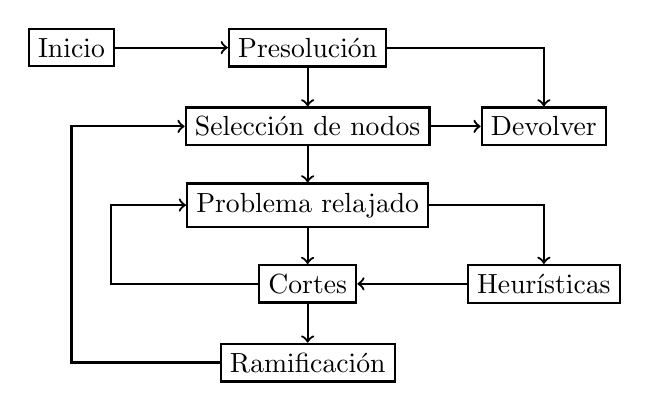
\begin{tikzpicture}[scale=1, node/.style={draw, thick}]
		\node[node] (Start) at (0,6) {Inicio};
		\node[node] (Presolve) at (3,6) {Presolución};
		\node[node] (Return) at (6,5) {Devolver};
		\node[node] (Node selection) at (3,5) {Selección de nodos};
		\node[node] (LP relaxation) at (3,4) {Problema relajado};
		\node[node] (Cuts) at (3,3) {Cortes};
		\node[node] (Branching) at (3,2) {Ramificación};
		\node[node] (Heuristics) at (6,3) {Heurísticas};
		% Arrows
		\draw[thick, ->] (Start) --(Presolve);
		\draw[thick, ->] (Presolve) -- (Node selection);
		\draw[thick, ->] (Presolve) -- (6,6) -- (Return);
		\draw[thick, ->] (Node selection) -- (LP relaxation);
		\draw[thick, ->] (Node selection) -- (Return);
		\draw[thick, ->] (LP relaxation) -- (Cuts);
		\draw[thick, ->] (LP relaxation) -- (6,4) -- (Heuristics);
		\draw[thick, ->] (Cuts) -- (Branching);
		\draw[thick, ->] (Heuristics) -- (Cuts);
		\draw[thick, ->] (Branching) -- (0,2) -- (0,5) --(Node selection);
		\draw[thick, ->] (Cuts) -- (0.5,3) -- (0.5,4) -- (LP relaxation);
	\end{tikzpicture} 
	\caption{Flujo típico de algoritmos que resuelven problemas lineales mixtos. Adaptado de
	\cite{fabs}.} \label{p1c11:fig:MIP_solver_flowchart}
\end{figure}

\begin{algorithm}[ht]
	\LinesNumbered
	\KwData{
		Problema de maximización lineal $S_0$.
		}
	\KwResult{
		Solución óptima entera $\vec{x}^*$ y valor óptimo $\optilp{z}$.
	}
	\Begin{
		$\mathcal{L} \leftarrow \braces{S_0}$\;
		$\vec{x}^* \leftarrow -\vec{\infty}$\;
		$\optilp{z} \leftarrow -\infty$\;
		\While{$\mathcal{L} \neq \emptyset$}{
			elegir de $\mathcal{L}$ subproblema $S_i$\; \nllabel{p1c9:alg:BB_loop}
			obtener de $S_i$ valor óptimo $z^*_i$ y solución óptima $\vec{x}^i$\;
			$\mathcal{L} \leftarrow \mathcal{L} \setminus \braces{S_i}$\;
			\If{$S_i = \emptyset$ o $z^*_i \leq \optilp{z}$}{
				ir al paso \eqref{p1c9:alg:BB_loop}\;
			}
			\If{$\vec{x}^i \in \Z^n$}{
				$\vec{x}^* \leftarrow \vec{x}^i$\;
				$\optilp{z} \leftarrow z^*_i$\;
				ir al paso \eqref{p1c9:alg:BB_loop}\;
			}
		    elegir $x^i_j \not \in \Z$ y generar subproblemas $S_{i0}$ y $S_{i1}$ con
			regiones factibles
			$S_{i} \cup \braces{x_j \leq \floor{x^i_j}}$ y
			$S_{i} \cup \braces{x_j \geq \ceil{x^i_j}}$, respectivamente\; \label{p1c9:alg:branch}
			$\mathcal{L} \leftarrow \mathcal{L} \cup \braces{S_{i1}, S_{i2}}$.
		}
		\Return{$(\vec{x}^*, \optilp{z})$}
	}
	\caption{Algoritmo de Ramificación y Acotamiento. Adaptado de \cite{fabs}.} \label{p1c9:alg:BB}
	\label{algo:bb}
\end{algorithm}
